\documentclass[serif]{beamer}\usepackage[]{graphicx}\usepackage[]{color}
%% maxwidth is the original width if it is less than linewidth
%% otherwise use linewidth (to make sure the graphics do not exceed the margin)
\makeatletter
\def\maxwidth{ %
  \ifdim\Gin@nat@width>\linewidth
    \linewidth
  \else
    \Gin@nat@width
  \fi
}
\makeatother

\definecolor{fgcolor}{rgb}{0.345, 0.345, 0.345}
\newcommand{\hlnum}[1]{\textcolor[rgb]{0.686,0.059,0.569}{#1}}%
\newcommand{\hlstr}[1]{\textcolor[rgb]{0.192,0.494,0.8}{#1}}%
\newcommand{\hlcom}[1]{\textcolor[rgb]{0.678,0.584,0.686}{\textit{#1}}}%
\newcommand{\hlopt}[1]{\textcolor[rgb]{0,0,0}{#1}}%
\newcommand{\hlstd}[1]{\textcolor[rgb]{0.345,0.345,0.345}{#1}}%
\newcommand{\hlkwa}[1]{\textcolor[rgb]{0.161,0.373,0.58}{\textbf{#1}}}%
\newcommand{\hlkwb}[1]{\textcolor[rgb]{0.69,0.353,0.396}{#1}}%
\newcommand{\hlkwc}[1]{\textcolor[rgb]{0.333,0.667,0.333}{#1}}%
\newcommand{\hlkwd}[1]{\textcolor[rgb]{0.737,0.353,0.396}{\textbf{#1}}}%
\let\hlipl\hlkwb

\usepackage{framed}
\makeatletter
\newenvironment{kframe}{%
 \def\at@end@of@kframe{}%
 \ifinner\ifhmode%
  \def\at@end@of@kframe{\end{minipage}}%
  \begin{minipage}{\columnwidth}%
 \fi\fi%
 \def\FrameCommand##1{\hskip\@totalleftmargin \hskip-\fboxsep
 \colorbox{shadecolor}{##1}\hskip-\fboxsep
     % There is no \\@totalrightmargin, so:
     \hskip-\linewidth \hskip-\@totalleftmargin \hskip\columnwidth}%
 \MakeFramed {\advance\hsize-\width
   \@totalleftmargin\z@ \linewidth\hsize
   \@setminipage}}%
 {\par\unskip\endMakeFramed%
 \at@end@of@kframe}
\makeatother

\definecolor{shadecolor}{rgb}{.97, .97, .97}
\definecolor{messagecolor}{rgb}{0, 0, 0}
\definecolor{warningcolor}{rgb}{1, 0, 1}
\definecolor{errorcolor}{rgb}{1, 0, 0}
\newenvironment{knitrout}{}{} % an empty environment to be redefined in TeX

\usepackage{alltt}
\usetheme{Boadilla}
\usepackage{graphicx}
\usepackage[draft]{animate}
\usepackage{breqn}
\usepackage{xcolor}
\usepackage{booktabs}
\usepackage{tikz}
\usetikzlibrary{decorations.pathreplacing}
\usetikzlibrary{shapes,arrows,positioning,shadows}
\usepackage{subfig}
\usepackage{pgf}

% change format of enumerated lists
\setbeamertemplate{enumerate items}[default]

\setbeamertemplate{navigation symbols}{}

% custom colors
\definecolor{mypal1}{HTML}{F0F9E8}\definecolor{mypal2}{HTML}{BAE4BC}\definecolor{mypal3}{HTML}{7BCCC4}\definecolor{mypal4}{HTML}{43A2CA}\definecolor{mypal5}{HTML}{0868AC}

\tikzstyle{decision} = [diamond, draw, text width=6em, text badly centered, inner sep = 2pt, top color=white, bottom color=mypal3, drop shadow]
\tikzstyle{block} = [rectangle, draw, text width=10em, text centered, rounded corners, minimum height=3em, minimum width=8em, top color = white, bottom color=mypal4,  drop shadow]
\tikzstyle{declare} = [rectangle, draw, text width=10em, text centered, minimum height=3em, minimum width=8em, top color = white, bottom color=mypal5,  drop shadow]

% knitr setup


% dependent data


% get online bib file


% my custom ggplot theme


% figure used on title page


\setbeamercolor{title}{fg=mypal5} % main title
\setbeamercolor{frametitle}{fg=mypal4, bg=mypal2} % frame titles
\setbeamercolor{structure}{fg=mypal4} % bottom banner
\setbeamercolor{normal text}{fg=mypal5}
\usebackgroundtemplate{
\includegraphics[height=\paperheight,width=\paperwidth]{fig/back_tmp.pdf}}

% macros
\newcommand{\emtxt}[1]{\textbf{\textit{#1}}}
\IfFileExists{upquote.sty}{\usepackage{upquote}}{}
\begin{document}

\title[Evaluating water quality]{\textbf{Quantitative approaches to evaluate surface water quality: Examples from Minnesota Lakes to Florida Estuaries}}
\author[M. Beck]{Marcus W. Beck}

\institute[USEPA]{ORISE post-doc, USEPA National Health and Environmental Effects Research Laboratory, Gulf Ecology Division, \href{mailto:beck.marcus@epa.gov}{beck.marcus@epa.gov}, Phone: 8509342480}

\date{Sep. 22, 2015}

\titlegraphic{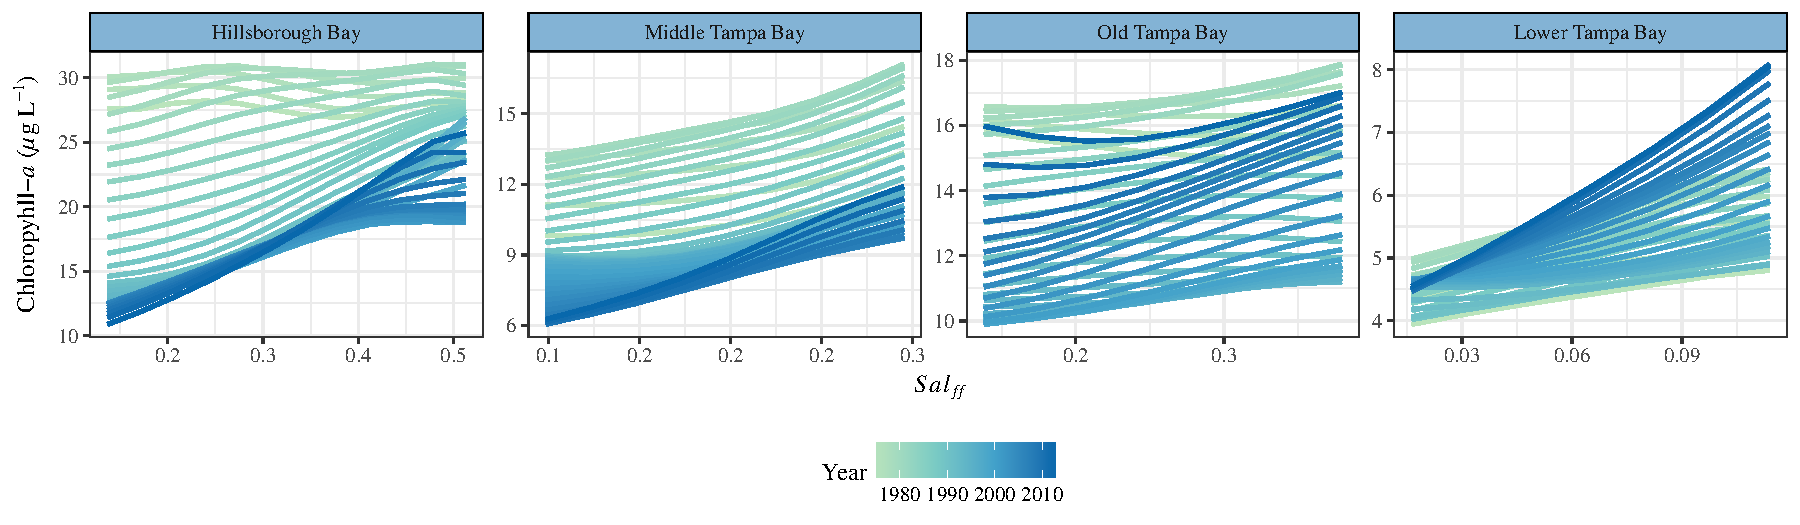
\includegraphics[width=0.95\linewidth]{fig/title_plo.pdf}}

%%%%%%
\begin{frame}[shrink]
\titlepage
\end{frame}

\section{Background}

%%%%%%
\begin{frame}{\textbf{Assessing environmental condition}}{\textbf{How do we collect and use data?}}
\onslide<+->
The foundation of environmental management is a strong monitoring network \scriptsize \cite{NRC90}\\~\\
\normalsize
Monitoring provides information for decision-making based on apparent trends...
\vspace{0.2in}
\begin{center}
\emtxt{What are the changes in environmental condition over time?}\\~\\
\emtxt{Are these changes `good' or `bad' based on our management objectives?}\\~\\
\emtxt{What may have caused these changes?}
\end{center}
\end{frame}

%%%%%%
\begin{frame}{\textbf{Assessing environmental condition}}{\textbf{How do we collect and use data?}}
\onslide<+->
\emtxt{The good news}: We are getting better at monitoring - standardized, automated, increased coverage, real-time/continuous \\~\\
\emtxt{The bad news}: Our ability to use these data for decision-making has not kept pace with availability! \\~\\
\onslide<+->


{\centering 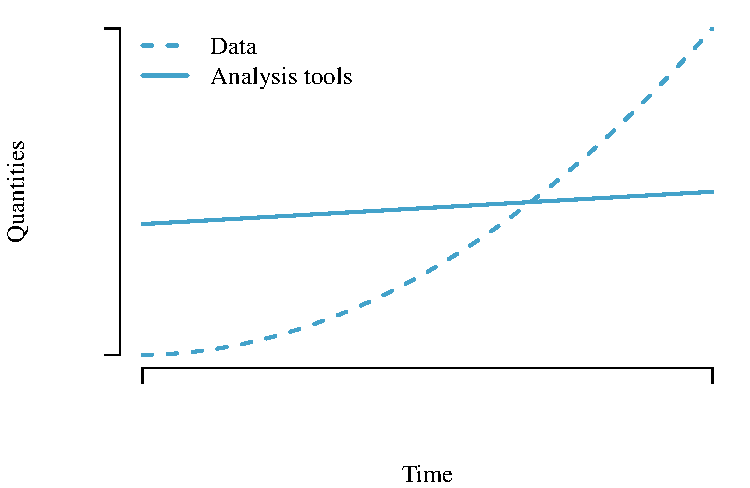
\includegraphics[width=0.55\textwidth]{fig/theo-1} 

}



\end{frame}

%%%%%%
\begin{frame}{\textbf{Assessing environmental condition}}{\textbf{How do we collect and use data?}}
Most of my research career has focused on using monitoring data to understand effects of eutrophication in one form or another \\~\\
\onslide<+->
\begin{quote}
Eutrophication (noun) - an \emtxt{increase} in the rate of supply of \emtxt{organic matter} to an ecosystem\\
\hfill -- \cite{Nixon95}
\end{quote}
\begin{center}
\scalebox{1}{
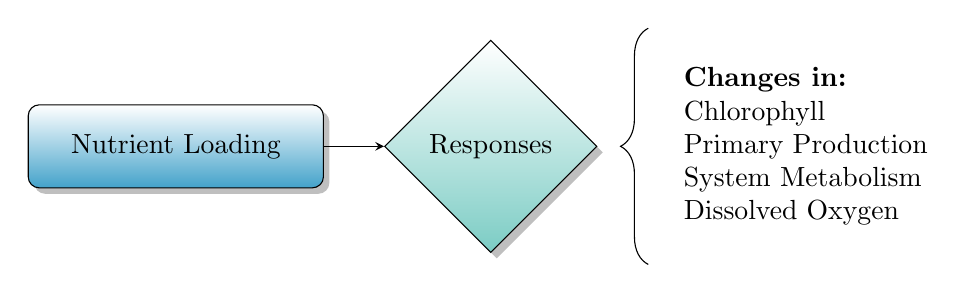
\begin{tikzpicture}[node distance = 4cm, auto, >=stealth]
  \onslide<+->{
  \node[block] (a) {Nutrient Loading};}
  \onslide<+->{
	\node[decision] (b)  [right of=a] {Responses};
 	\draw[->] (a) -- (b);}
  \onslide<+->{
  \draw[decorate,decoration={brace,amplitude=10pt}] [right of=b] (2,-1.5) -- (2,1.5);
  \node[draw,align=left,draw=none] [right of=b] {\textbf{Changes in:}\\ Chlorophyll\\ Primary Production\\ System Metabolism\\ Dissolved Oxygen};}
\end{tikzpicture}}
\end{center}
\vspace{-0.5cm}\hspace*{15pt}\scalebox{0.7}{\hbox{\tiny Adapted from \cite{Cloern01}}}\\~\\
\end{frame}

%%%%%%
\begin{frame}{\textbf{Assessing environmental condition}}{\textbf{How do we collect and use data?}}
\onslide<+->
Today's talk: My experience synthesizing and evaluating monitoring data to inform our understanding of the eutrophication paradigm\\~\\
\begin{itemize}
\item \emtxt{Case 1}: Understanding response of a biotic index for Minnesota lakes \\~\\
\item \emtxt{Case 2}: Evaluating long-term datasets of chlorophyll in Tampa Bay \\~\\
\item \emtxt{Case 3}: Development of `open-science' tools for the National Estuarine Research Reserve System \\~\\
\end{itemize}
\onslide<+->
Each case addresses the challenges of \emtxt{understanding nutrient dynamics} and \emtxt{developing quantitative tools} for assessment
\end{frame}

\section{Case 1: Minnesota lakes}

%%%%%%
\begin{frame}{\textbf{Case 1: Minnesota lakes}}{\textbf{Evaluating biological response}}
\begin{columns}
\begin{column}{0.5\textwidth}
\centerline{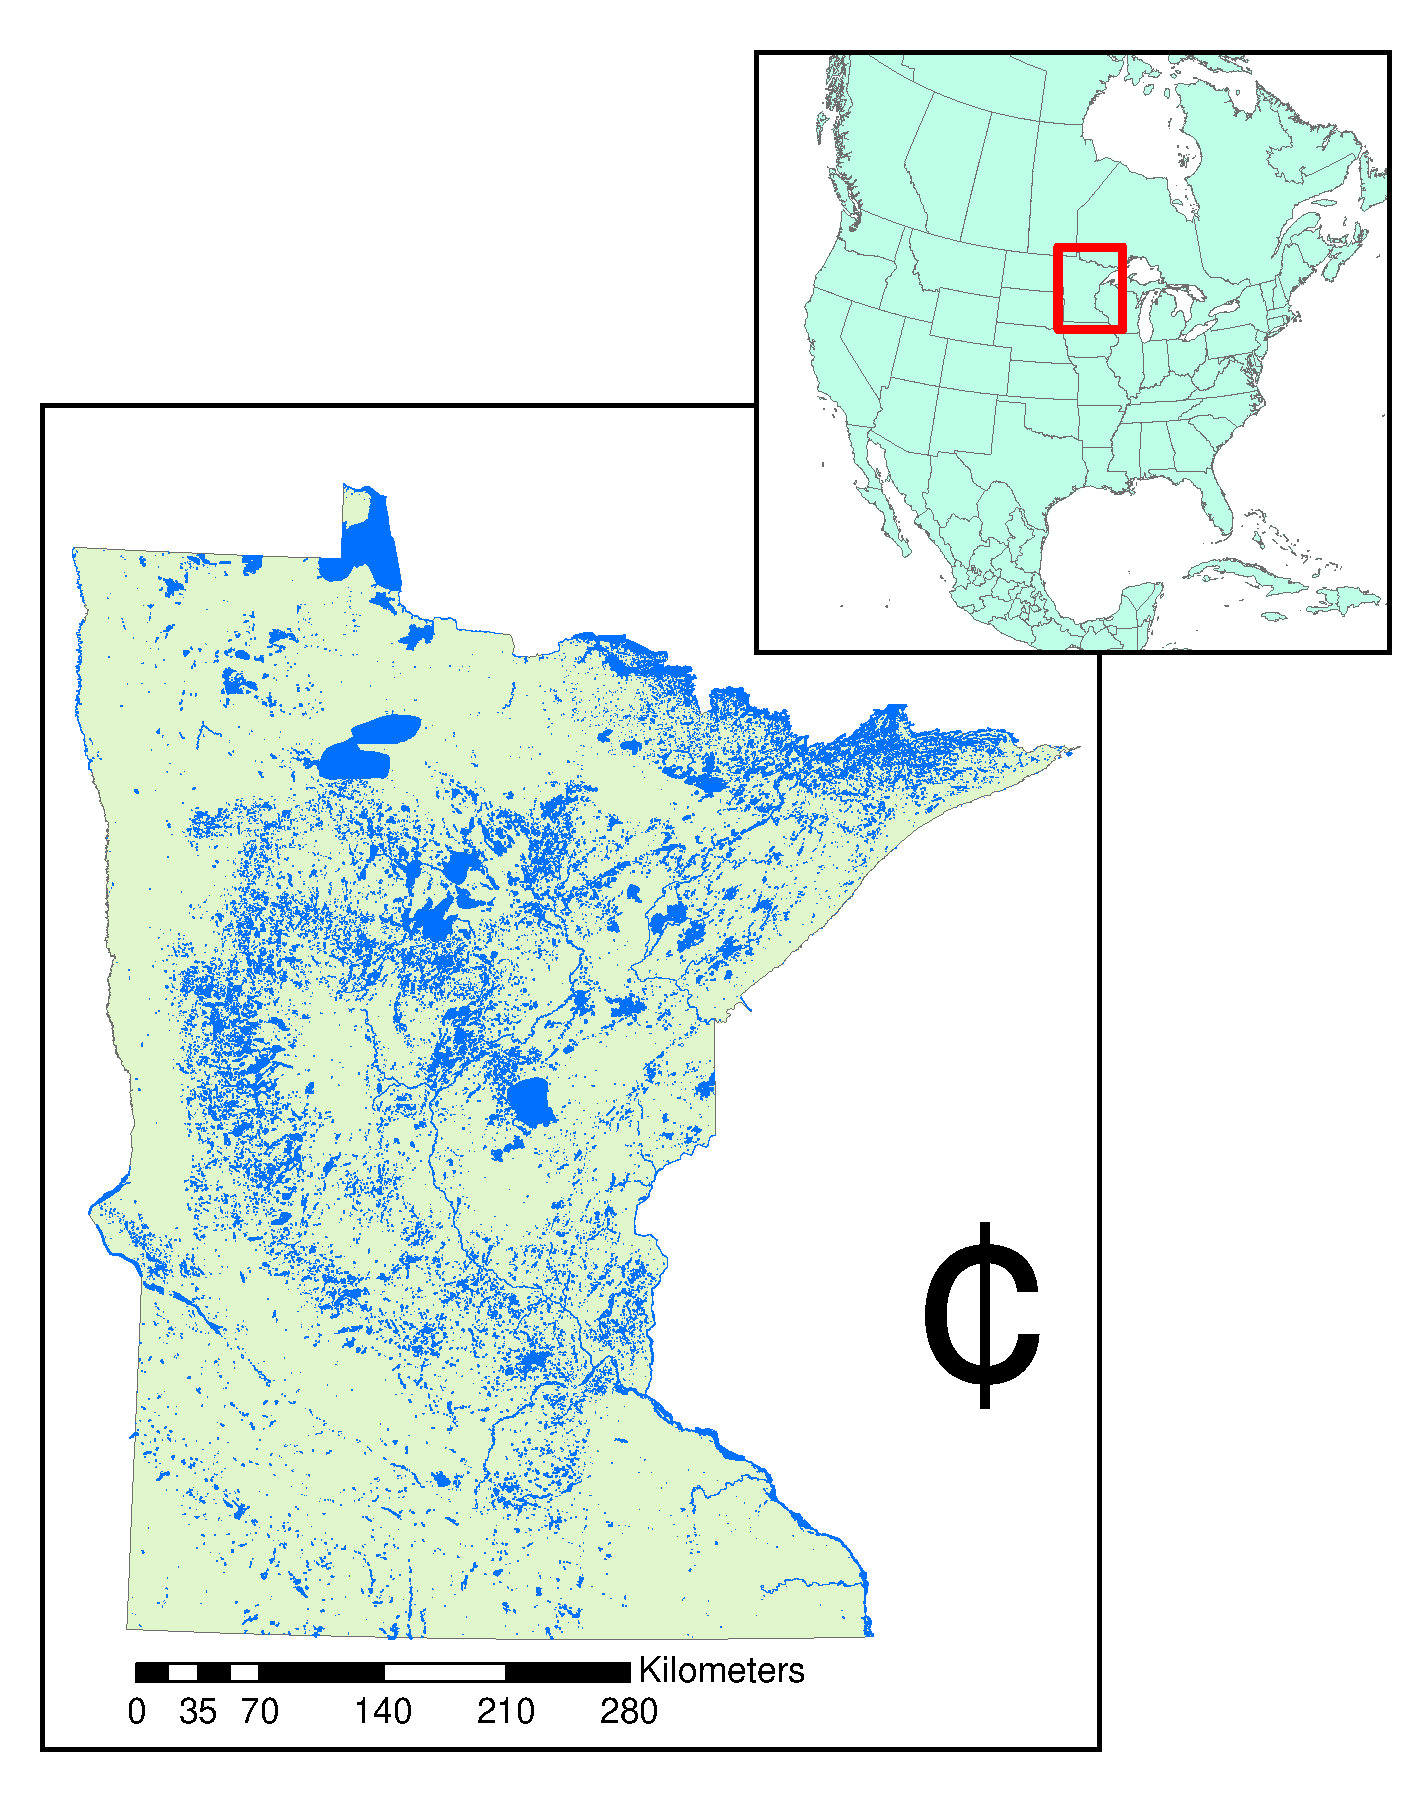
\includegraphics[width=\textwidth]{fig/mn_lake_inset.pdf}}
\end{column}
\begin{column}{0.5\textwidth}
\begin{center}

\includegraphics[width=0.5\textwidth]{fig/mn_seal.jpg} \\~\\
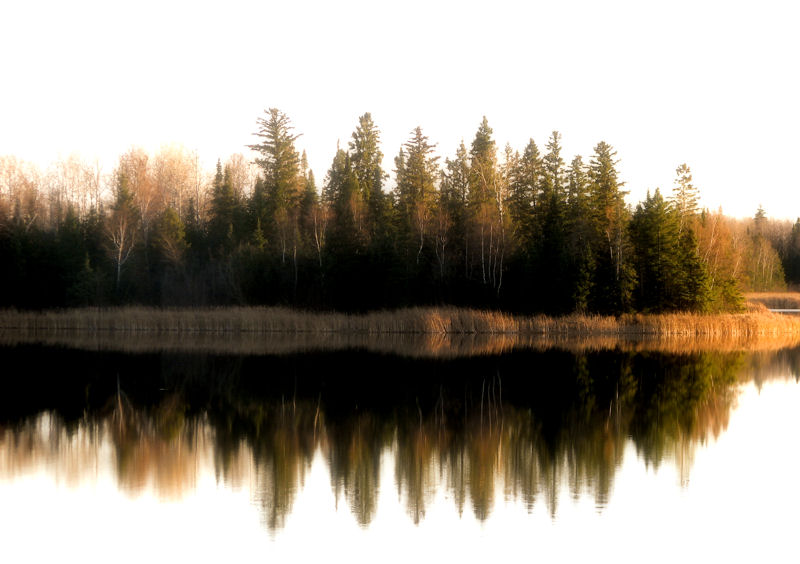
\includegraphics[width=0.9\textwidth]{fig/mn_lake.jpg}
\end{center}
\end{column}
\end{columns}
\end{frame}

%%%%%%
\begin{frame}{\textbf{Case 1: Minnesota lakes}}{\textbf{Evaluating biological response}}
\centerline{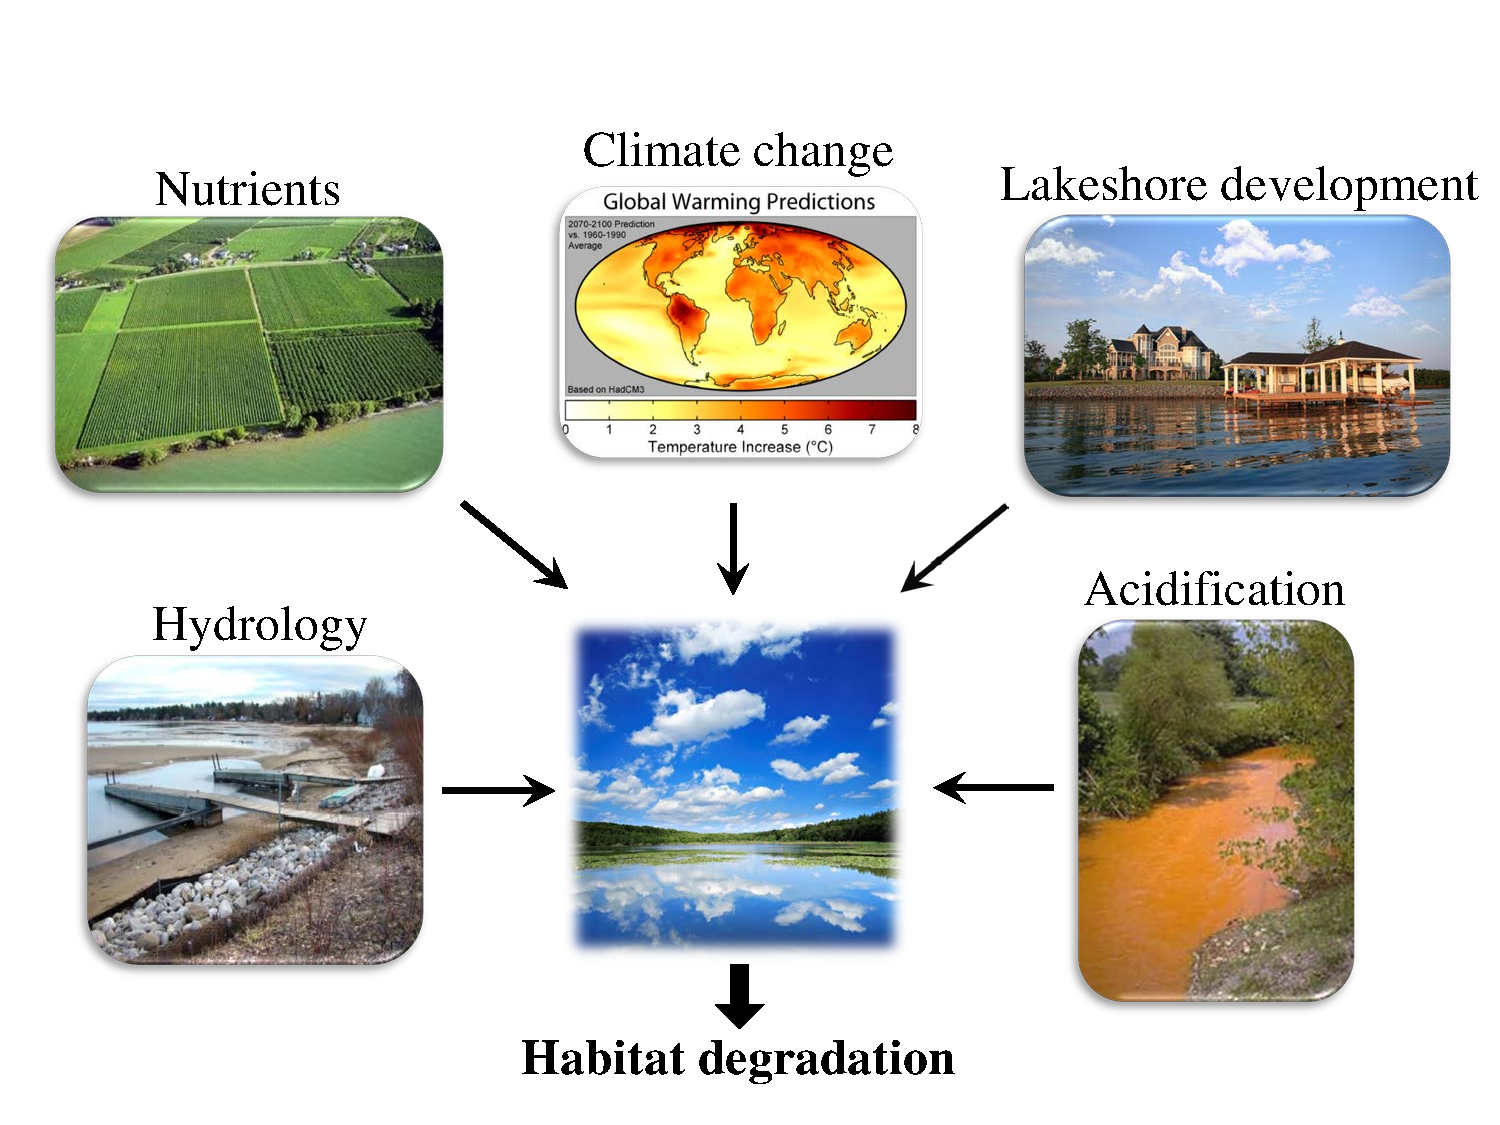
\includegraphics[width=0.9\textwidth]{fig/stressors.pdf}}
\end{frame}

%%%%%%
\begin{frame}{\textbf{Case 1: Minnesota lakes}}{\textbf{Evaluating biological response}}
\onslide<+->
Water Quality Act Amendments of 1972
\begin{itemize}
\item{Federal mandates to protect and restore the chemical, physical, and \emtxt{biological} integrity of surface waters}
\item{Protection and restoration requires monitoring \\~\\}
\end{itemize}
\onslide<+->
Index of biotic integrity (IBI) \cite{Karr81,Karr86}
\begin{itemize}
\item{Monitoring framework for definition and evaluation of biotic integrity}
\item{Uses aquatic organisms as indicators of ecosystem health}
\item{A multimetric index that is regionally specific}
\end{itemize}
\end{frame}

%%%%%%
\begin{frame}{\textbf{Case 1: Minnesota lakes}}{\textbf{Evaluating biological response}}
\onslide<+->
The macrophyte IBI can be used to evaluate relative lake condition by monitoring and evaluating aquatic plant metrics \cite{Beck10} \\~\\
\onslide<+->
Composed of eight metrics, summed to get one IBI score per lake \\~\\
\begin{itemize}
\item{MAXD: Maximum depth of plant growth}
\item{LITT: Percentage of littoral zone vegetated}
\item{OVER: Number of species with frequency occurrence $>$10\%}
\item{EMFL: Relative frequency of emergent-floating species}
\item{SUBM: Relative frequency of submersed species}
\item{SENS: Relative frequency of sensitive species}
\item{TOLR: Relative frequency of tolerant species}
\item{TAXA: Number of native taxa \\~\\}
\end{itemize}
\end{frame}

%%%%%%
\begin{frame}{\textbf{Case 1: Minnesota lakes}}{\textbf{Evaluating biological response}}
\begin{columns}
\onslide<+->
\begin{column}{0.5\textwidth}
\begin{center}
Related to changes in water quality \\~\\
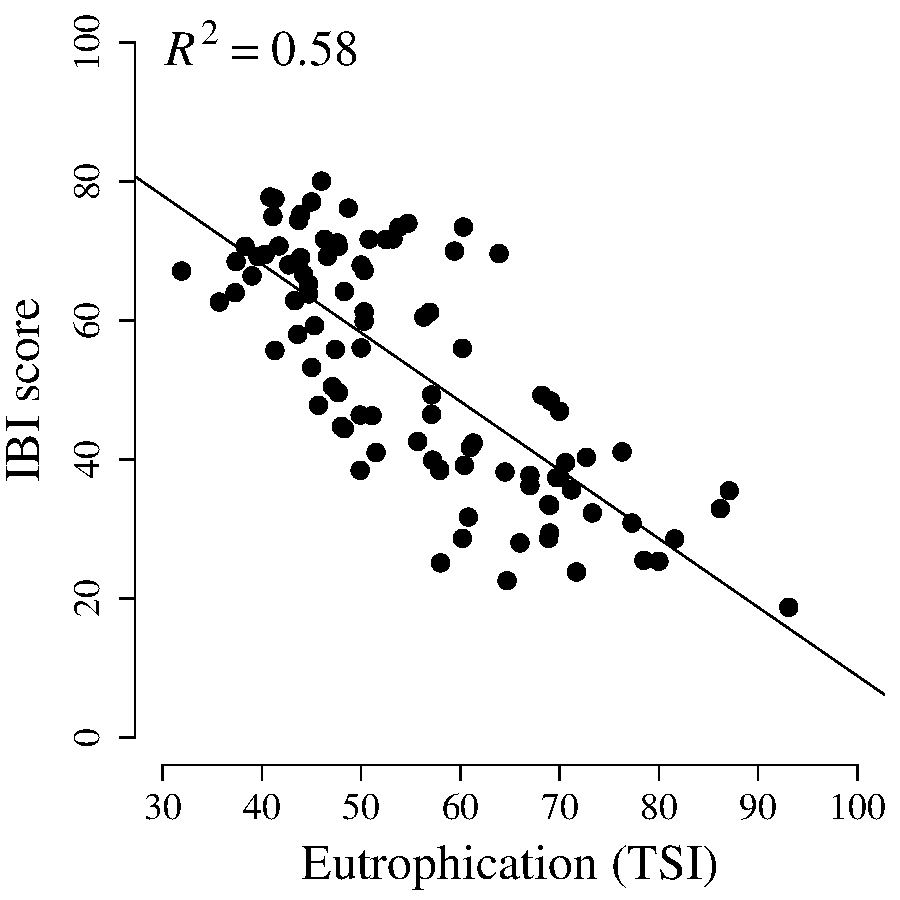
\includegraphics[width=\textwidth]{fig/Beck_GEDsem-ibi_tsi.pdf}
\end{center}
\end{column}
\onslide<+->
\begin{column}{0.5\textwidth}
\begin{center}
High precision given sampling effort \\~\\
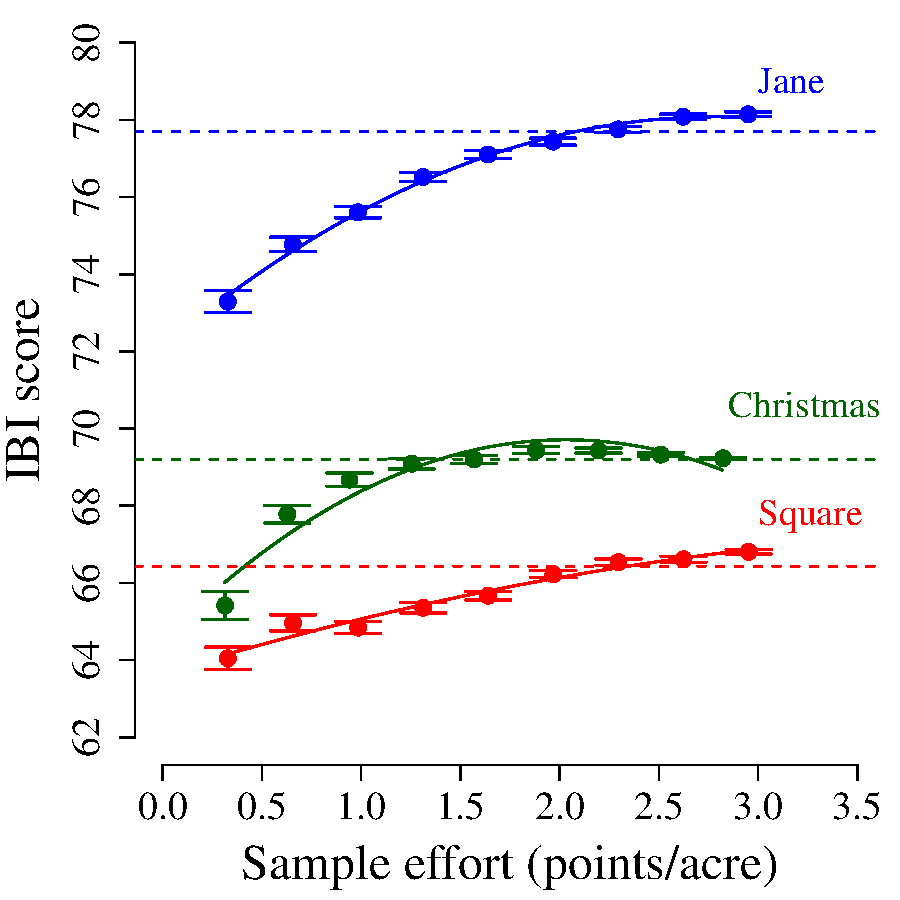
\includegraphics[width=\textwidth]{fig/Beck_GEDsem-ibi_eff.pdf}
\end{center}
\end{column}
\end{columns}
\end{frame}

%%%%%%
\begin{frame}{\textbf{Case 1: Minnesota lakes}}{\textbf{Evaluating biological response}}
\onslide<+->{How appropriate is the IBI for characterizing effects of multiple stressors? Will it work within an assessment/impairment framework?\\~\\}
\onslide<+->{
\vspace*{-0.1in}
\begin{center}
\scalebox{0.8}{
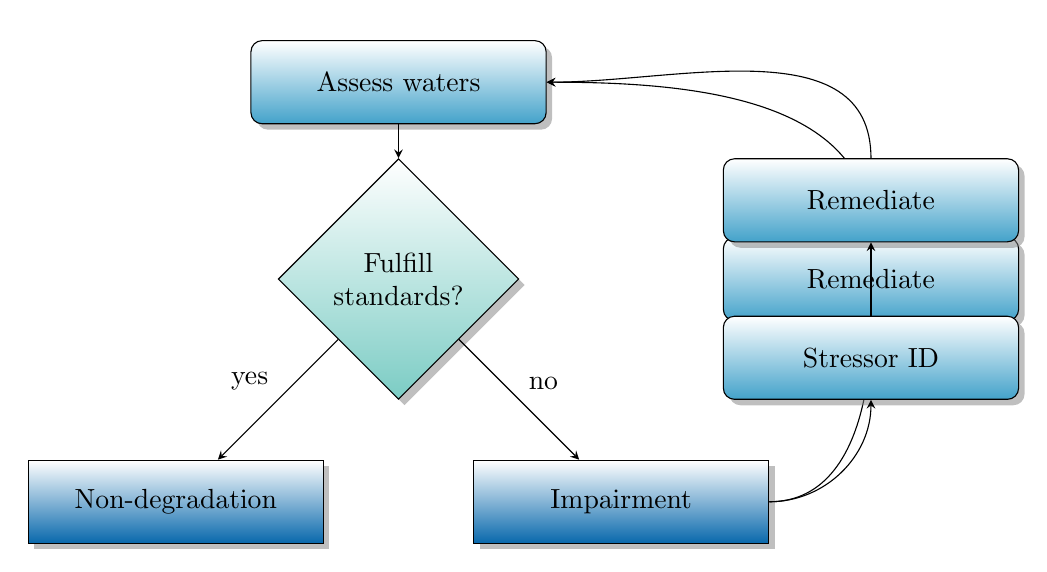
\begin{tikzpicture}[node distance=2.5cm, auto, >=stealth]
	\node[block] (a) {Assess waters};
	\onslide<+->{
	\node[decision] (b)  [below of=a] {Fulfill standards?};
 	\draw[->] (a) -- (b);}
 	\onslide<+->{
 	\node[declare] (c)  [below left of=b, node distance=4cm]  {Non-degradation};
 	\draw[->] (b) -- node[above left] {yes} (c);}
 	\onslide<+->{
 	\node[declare] (d)  [below right of=b, node distance=4cm]  {Impairment};
 	\draw[->] (b) -- node[above right] {no} (d);}
 	\onslide<+>{
 	\node[block] (e)  [right of=b, node distance=6cm]    {Remediate};
 	\draw[->] (d.east) to [out=360,in=270] (e.south);
 	\draw[->] (e.north) to [out=90,in=360] (a.east);}
 	\onslide<+->{
 	\node[block] (f)  [below of=e, node distance=1cm]    {Stressor ID};
 	\node[block] (g)  [above of=e, node distance=1cm]    {Remediate};
	\draw[->] (d.east) to [out=360,in=270] (f.south);
	\draw[->] (f.north) to [out=90,in=270] (g.south);
 	\draw[->] (g.north) to [out=90,in=360] (a.east);}
\end{tikzpicture}}
\end{center}}
\end{frame}

%%%%%%
\begin{frame}{\textbf{Case 1: Minnesota lakes}}{\textbf{Evaluating biological response}}
\onslide<+->
Consider an IBI with 12 metrics, each scored 1, 3, or 5\\~\\
How many different combinations of metrics lead to the same score?
\onslide<+->


{\centering 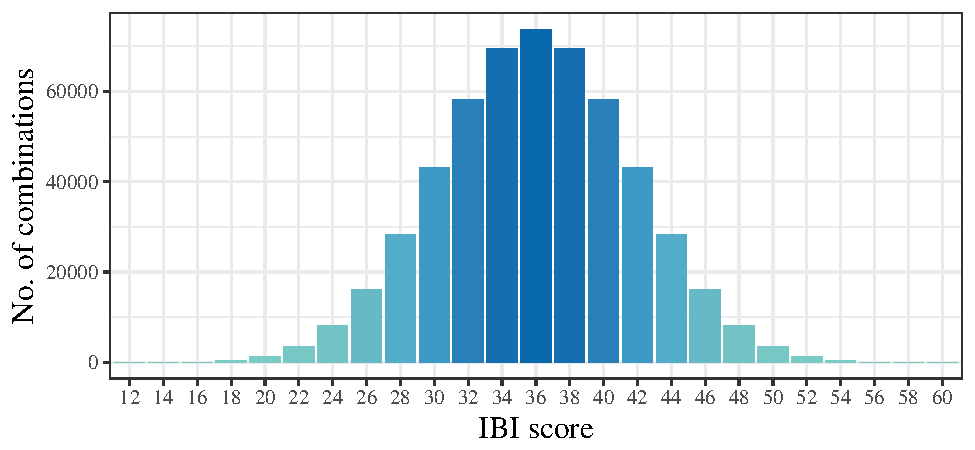
\includegraphics[width=\maxwidth]{fig/ibi_comb-1} 

}



\end{frame}

%%%%%%
\begin{frame}{\textbf{Case 1: Minnesota lakes}}{\textbf{Evaluating biological response}}
\onslide<+->
\textbf{\emph{Develop and implement a framework for evaluating the macrophyte IBI to inform its use in biological monitoring:}} \\~\\
\begin{enumerate}
\onslide<+->
\item How well does the index distinguish between signal and noise? \\~\\
\onslide<+->
\item Can information on stressors and their effects be quantified with certainty? \\~\\
\onslide<+->
\item What stressors primarily influence index response? \\~\\
\onslide<+->
\item How appropriate is a multimetric index for characterizing effects of multiple stressors?
\end{enumerate}
\end{frame}

%%%%%%
\begin{frame}{\textbf{Case 1: Minnesota lakes}}{\textbf{Evaluating biological response}}
\begin{itemize}
\item Dataset of 332 vegetation surveys, courtesy of MNDNR
\item Numerous covariates describing lake characteristics and anthropogenic stressors
\end{itemize}
\begin{columns}
\begin{column}{0.5\textwidth}
\centerline{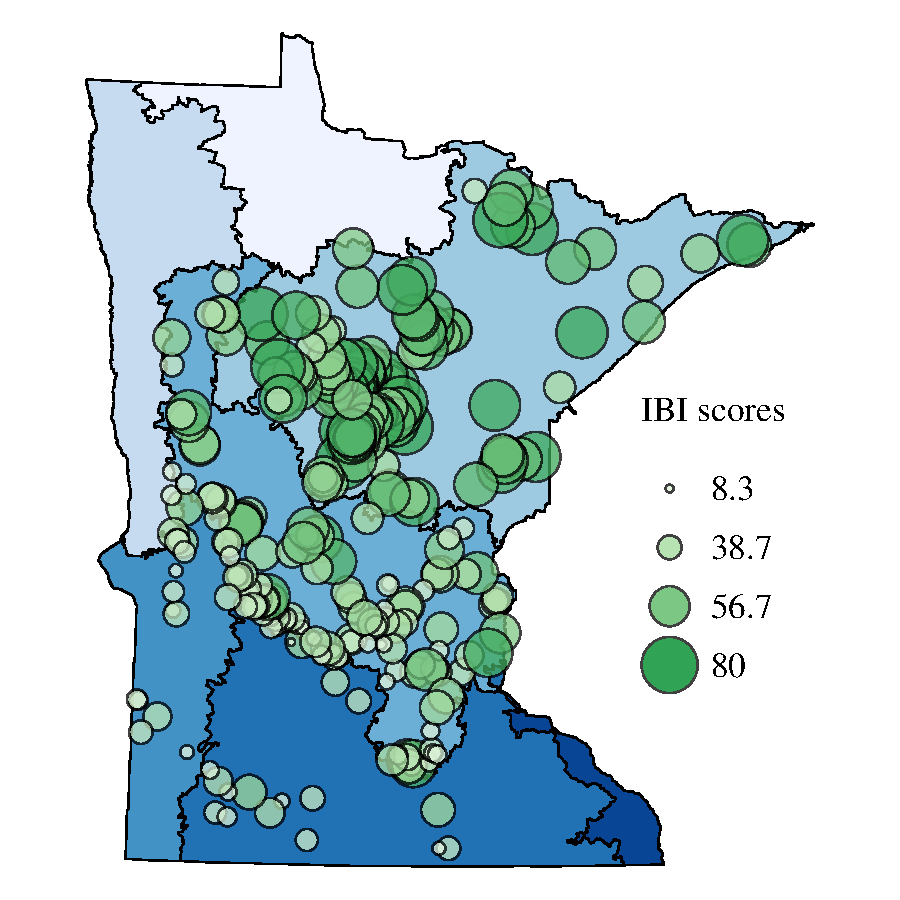
\includegraphics[width=\textwidth]{fig/Beck_GEDsem-ibi_data.pdf}}
\end{column}
\begin{column}{0.5\textwidth}
\scriptsize
\begin{itemize}
\item{lake surface area}
\item{maximum lake depth}
\item{trophic state index}
\item{growing degree days}
\item{percent agriculture in wshed}
\item{percent impervious surfaces in wshed}
\item{density of groundwater wells in wshed}
\item{wshed area to lake area}
\item{crop productivity index of wshed}
\item{dock density}
\item{...}
\end{itemize}
\end{column}
\end{columns}
\end{frame}

%%%%%%
\begin{frame}{\textbf{Case 1: Minnesota lakes}}{\textbf{Evaluating biological response}}
\onslide<+->
Ecological and numerical complexity warrants the use of creative solutions\\~\\
Neural networks to model IBI response\\~\\
\begin{itemize}
\onslide<+->
\item{Essentially a large, non-linear regression model free of assumptions that can handle multivariate response}
\onslide<+->
\item{Models relationships among variables using a network that mimics neuronal structure of the human brain}
\onslide<+->
\item{`Supervised' neural networks are meant for prediction but network information can be used to infer causation}
\end{itemize}
\end{frame}

%%%%%%
\begin{frame}{\textbf{Case 1: Minnesota lakes}}{\textbf{Evaluating biological response}}
\begin{center}
\animategraphics[controls, width =.65\linewidth]{12}{fig/Rplot}{}{} %frame rate is 12 per/sec
\end{center}
\end{frame}

%%%%%%
\begin{frame}{\textbf{Case 1: Minnesota lakes}}{\textbf{Evaluating biological response}}
\begin{center}
\animategraphics[controls,width=0.85\linewidth]{12}{fig/train_iter}{}{}
\end{center}
\end{frame}

%%%%%%
\begin{frame}{\textbf{Case 1: Minnesota lakes}}{\textbf{Evaluating biological response}}
Modification of Garson's algorithm to determine relative importance of variables \cite{Garson91}
\begin{columns}
\begin{column}{0.5\textwidth}
\begin{center}
\includegraphics<1->[width=\textwidth,page=2]{fig/Beck_GEDsem-nnet_relimp1.pdf}
\end{center}
\end{column}
\begin{column}{0.5\textwidth}
\begin{center}
\includegraphics<1>[width=\textwidth,page=11]{fig/Beck_GEDsem-nnet_relimp2.pdf}
\includegraphics<2>[width=\textwidth,page=12]{fig/Beck_GEDsem-nnet_relimp2.pdf}
\includegraphics<3>[width=\textwidth,page=13]{fig/Beck_GEDsem-nnet_relimp2.pdf}
\includegraphics<4>[width=\textwidth,page=14]{fig/Beck_GEDsem-nnet_relimp2.pdf}
\includegraphics<5>[width=\textwidth,page=15]{fig/Beck_GEDsem-nnet_relimp2.pdf}
\includegraphics<6>[width=\textwidth,page=16]{fig/Beck_GEDsem-nnet_relimp2.pdf}
\includegraphics<7>[width=\textwidth,page=17]{fig/Beck_GEDsem-nnet_relimp2.pdf}
\includegraphics<8>[width=\textwidth,page=18]{fig/Beck_GEDsem-nnet_relimp2.pdf}
\includegraphics<9>[width=\textwidth,page=19]{fig/Beck_GEDsem-nnet_relimp2.pdf}
\includegraphics<10->[width=\textwidth,page=20]{fig/Beck_GEDsem-nnet_relimp2.pdf}
\end{center}
\end{column}
\end{columns}
\onslide<11>
Relative importance is summation of product of weights between layers
\end{frame}

%%%%%%
\begin{frame}{\textbf{Case 1: Minnesota lakes}}{\textbf{Evaluating biological response}}
\begin{center}
\begin{figure}[p]
\subfloat[IBI scores]{
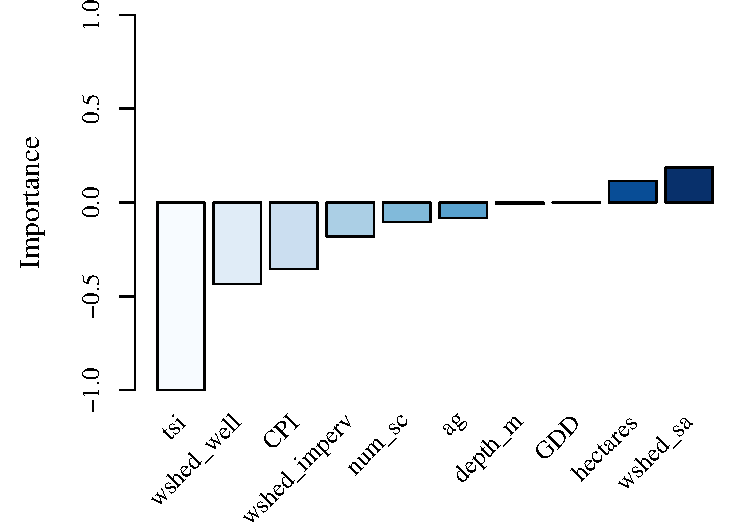
\includegraphics[width=0.5\textwidth,keepaspectratio=T,page=1]{fig/Beck_GEDsem-gar_exp_met.pdf}
}
\subfloat[MAXD metric]{
\includegraphics[width=0.5\textwidth,keepaspectratio=T,page=2]{fig/Beck_GEDsem-gar_exp_met.pdf}
}
\vspace{0.1in}
\caption{Examples of relative importance of explanatory variables based on weights between layers in optimal neural networks.}  
\end{figure}
\end{center}
\end{frame}

%%%%%%
\begin{frame}{\textbf{Case 1: Minnesota lakes}}{\textbf{Evaluating biological response}}
\onslide<+->
Neural networks are powerful enough to model noise in the data \\~\\
The model may be specific to peculiarities the training dataset \\~\\
Uncertainty of variable importance must be quantified - bootstrap! 
\onslide<+->
\begin{center}
\begin{figure}[t]
\subfloat{
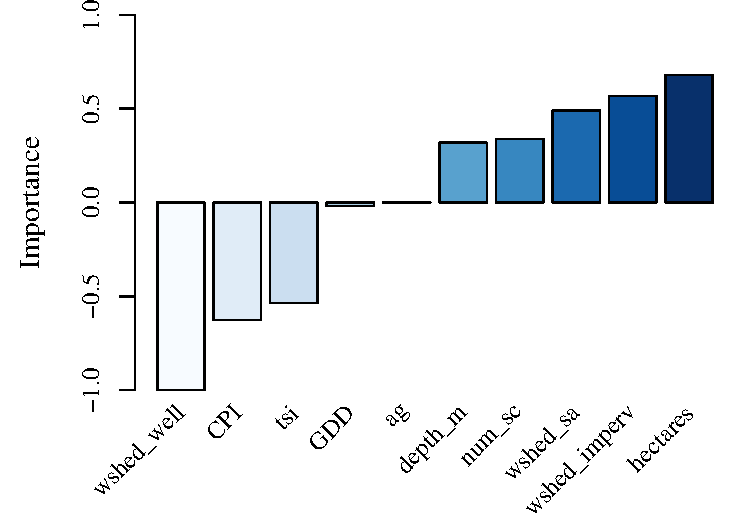
\includegraphics[width=0.5\textwidth,keepaspectratio=T,page=1]{fig/Beck_GEDsem-gar_boot.pdf}
}
\subfloat{
\includegraphics[width=0.5\textwidth,keepaspectratio=T,page=2]{fig/Beck_GEDsem-gar_boot.pdf}
}
\end{figure} %TAXA
\end{center}
\end{frame}

%%%%%%
\begin{frame}{\textbf{Case 1: Minnesota lakes}}{\textbf{Evaluating biological response}}
Lots of uncertainty associated with input contributions... \\~\\
\begin{itemize}
\item One of ten relationships for IBI scores with explanatory variables
\item Four of 80 relationships for metrics with explanatory variables
\pause
\item IBI negatively related to lake trophic state
\item MAXD, OVER, and TAXA negatively related to lake trophic state
\item TAXA positively related to lake size\\~\\
\end{itemize}
\pause
What is the source of this uncertainty? Sample sizes, method, neural network?
\end{frame}

%%%%%%
\begin{frame}{\textbf{Case 1: Minnesota lakes}}{\textbf{Evaluating biological response}}
Potentially competing objectives of an IBI: certainty vs simplicity \\~\\
\pause
\begin{quote}
IBI relies on multiparameters, a requirement when the system to be evaluated is complex. \cite{Karr86} \\~\\
\end{quote}
\begin{quote}
The resulting index allows people without specialized expertise to understand overall condition and to make informed decisions that will then affect the health of those resources. \cite{Karr99} \\~\\
\end{quote}
\pause
\begin{quote}
Combining responses into an index hides the component responses, thereby obscuring causation. \cite{Suter93}
\end{quote}
\end{frame}

%%%%%%
\begin{frame}{\textbf{Case 2: Florida estuaries}}{\textbf{Evaluating long-term chlorophyll datasets}}
USEPA Gulf Ecology Division - guidance to Florida DEP and others on criteria development for estuaries \\~\\
\centerline{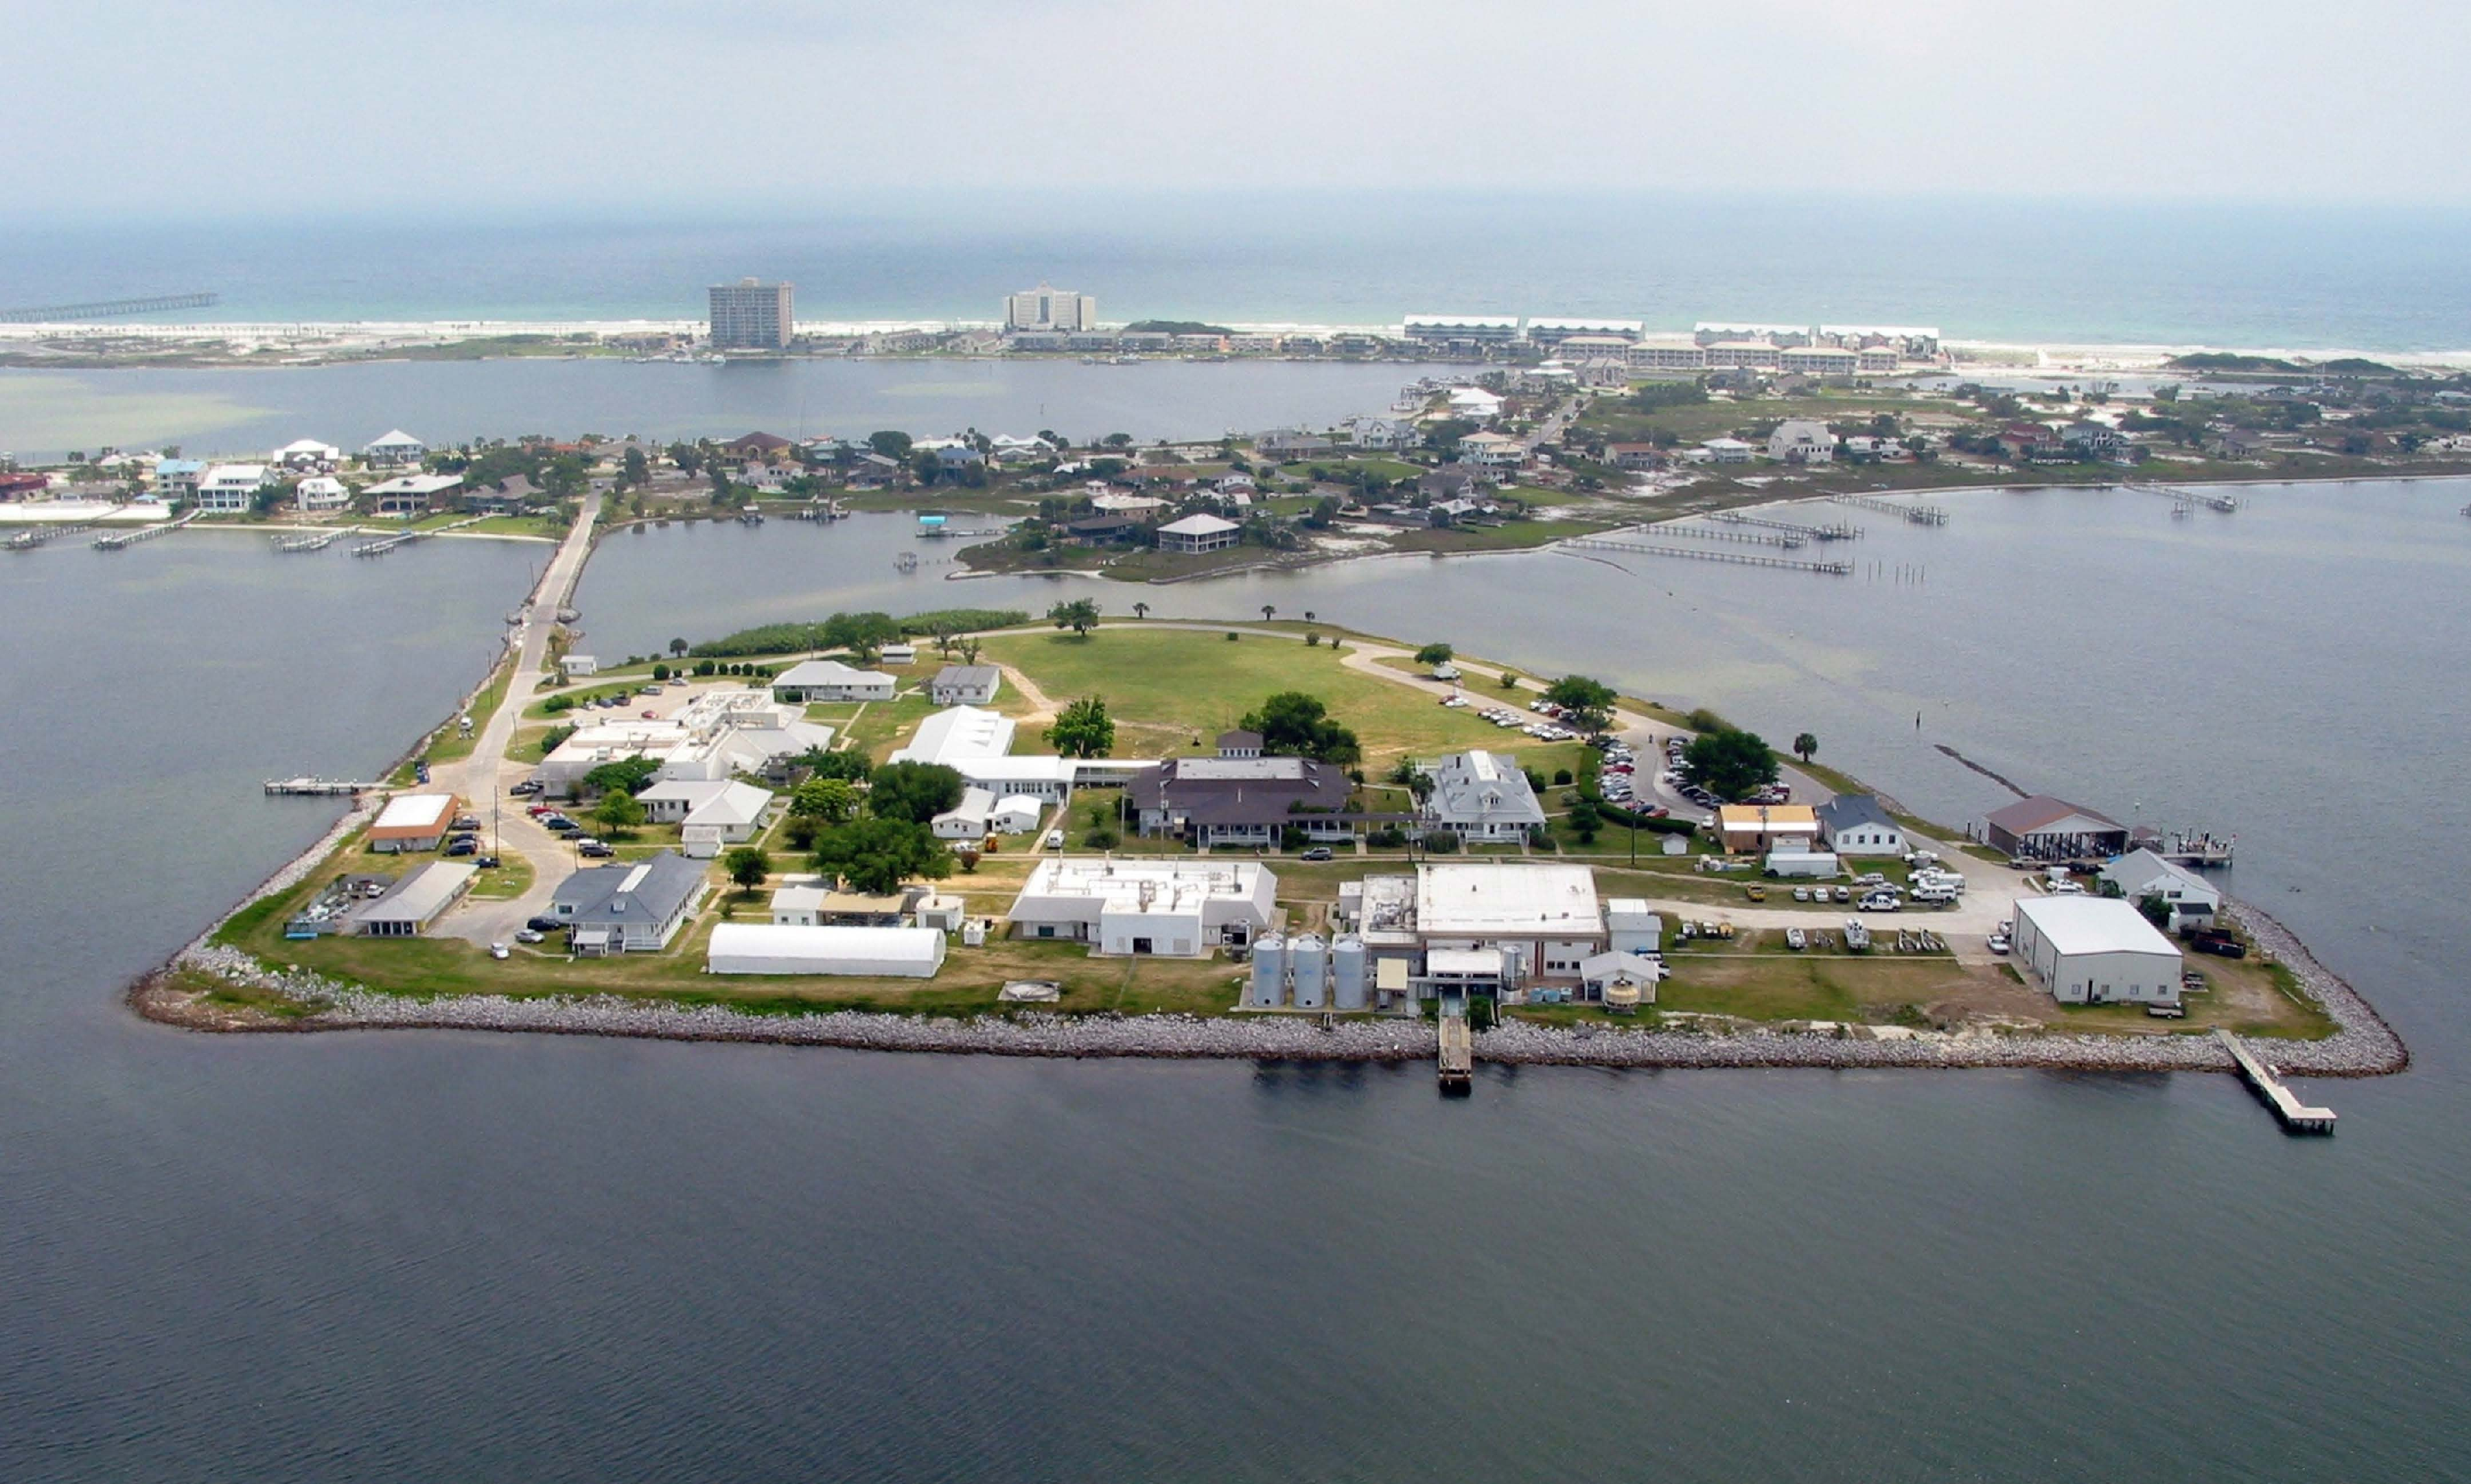
\includegraphics[width = 0.8\textwidth]{fig/sabine.pdf}}
\end{frame}

\section{Case 2: Florida Estuaries}

% tampa bay map, w/ inset


%%%%%%
\begin{frame}{\textbf{Case 2: Florida estuaries}}{\textbf{Evaluating long-term chlorophyll datasets}}
\begin{columns}
\begin{column}{0.5\textwidth}
\begin{itemize}
\item Four bay segments\\~\\
\item Monthly wq data at 50 stations from 1974 to present \\~\\
\item Longitudinal profile of nutrient load and salinity \\~\\
\end{itemize}
\vspace{0cm}\hspace*{15pt}\scalebox{0.7}{\hbox{\tiny Data from \cite{TBEP11}}}
\end{column}
\begin{column}{0.5\textwidth}
\centerline{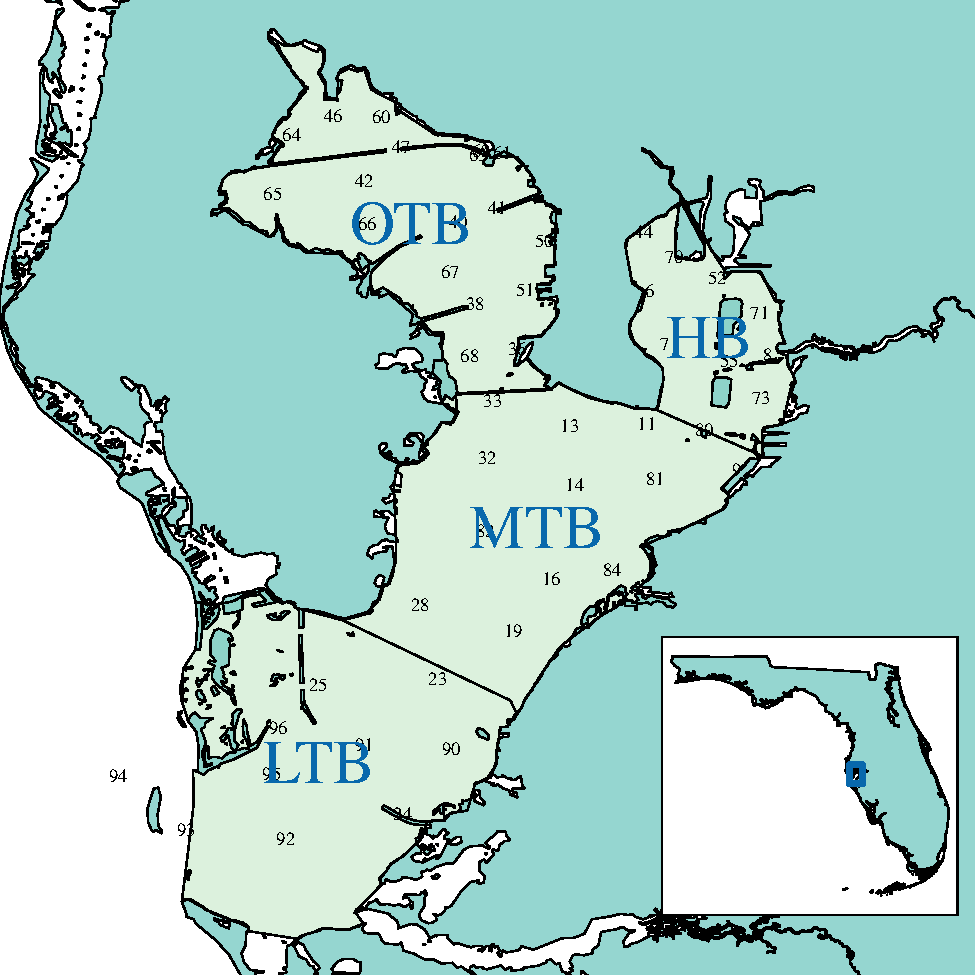
\includegraphics[width = \textwidth]{fig/tb_map.pdf}}
\end{column}
\end{columns}
\end{frame}

%%%%%%
\begin{frame}{\textbf{Case 2: Florida estuaries}}{\textbf{Evaluating long-term chlorophyll datasets}}
\begin{figure}[!ht]

{\centering 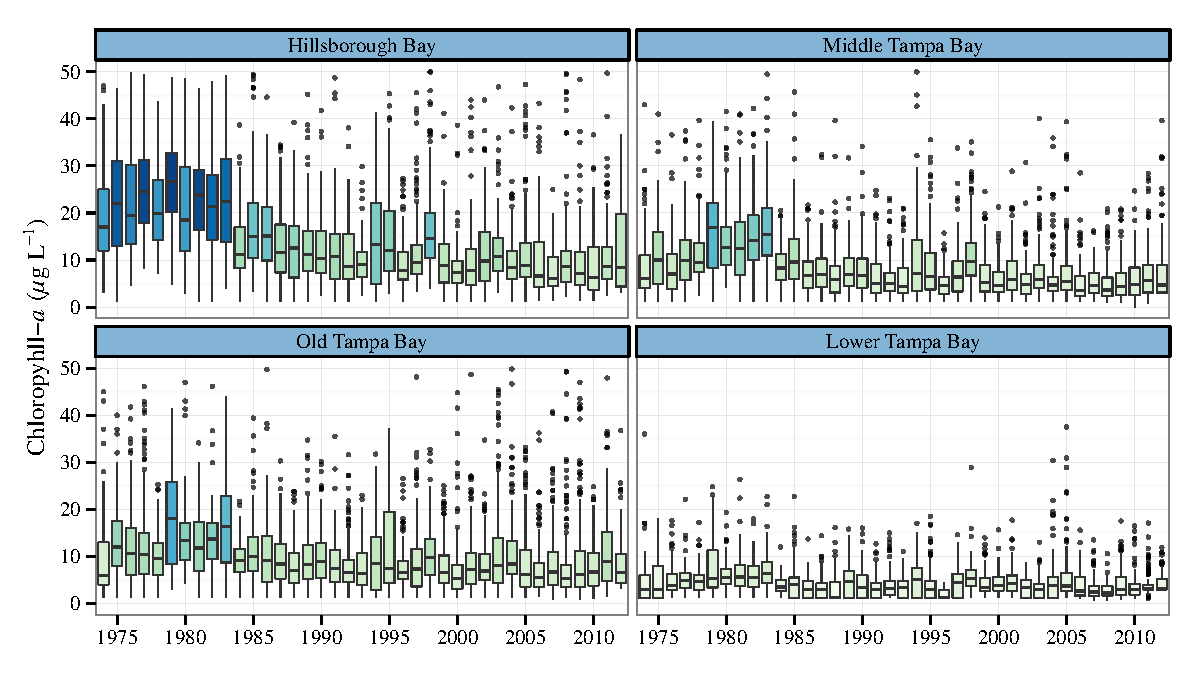
\includegraphics[width=\linewidth]{fig/annual_chl-1} 

}

\caption[Annual trends in chlorophyll for each bay segment]{Annual trends in chlorophyll for each bay segment.}\label{fig:annual_chl}
\end{figure}


\end{frame}

% variation in chl by year, season, and management

%%%%%%
\begin{frame}{\textbf{Case 2: Florida estuaries}}{\textbf{Evaluating long-term chlorophyll datasets}}
What affects our interpretation of chlorophyll response to nutrients?
\vspace{-0.1in}
\captionsetup[subfloat]{captionskip=0pt, position=top}
\begin{figure}
\centering
\subfloat[]{
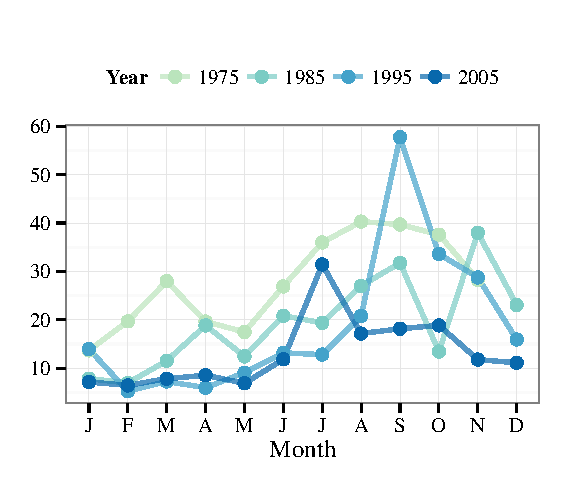
\includegraphics[width=0.46\textwidth,page=1,trim=0.2in 0in 0in 0.35in,clip]{fig/salmoyr.pdf}
\label{fig:salmoyr1}
}
\subfloat[]{
\includegraphics[width=0.46\textwidth,page=2,trim=0.2in 0in 0in 0.35in,clip]{fig/salmoyr.pdf}
\label{fig:salmoyr2}
}

\leavevmode\smash{\makebox[0pt]{\hspace{0em}% HORIZONTAL POSITION           
  \rotatebox[origin=l]{90}{\hspace{3em}% VERTICAL POSITION
    {\color{black} Chlorophyll-\textit{a}}}}}
    \hspace{0pt plus 1filll}\null

\caption{Variation in chlorophyll by {\color{mypal5}\protect\subref{fig:salmoyr1}} time and {\color{mypal5}\protect\subref{fig:salmoyr2}} salinity and management in Hillsborough Bay.  Panel {\color{mypal5}\protect\subref{fig:salmoyr1}} is colored before and after wastewater treatment in 1979.}
\label{fig:salmoyr}
\end{figure}
\captionsetup[subfloat]{position=top}
\end{frame}

%%%%%%
\begin{frame}{\textbf{Case 2: Florida estuaries}}{\textbf{Evaluating long-term chlorophyll datasets}}
\onslide<+->
\begin{block}{Study objective}
Adapt and apply nutrient response model for estuaries that leverages the descriptive capabilities of large datasets \scriptsize \cite{Beck15}
\end{block}
\vspace{0.2in}
\onslide<+->
Questions of concern -- Can we...
\begin{itemize}
\item ...provide a natural history of water quality that is temporally consistent with drivers of change?
\onslide<+->
\item ...characterize changes in extreme events in addition to describing the mean response?  
\onslide<+->
\item ...improve our understanding of the nutrient-response paradigm in estuaries?
\end{itemize}
\end{frame}

%%%%%%
\begin{frame}{\textbf{Case 2: Florida estuaries}}{\textbf{Evaluating long-term chlorophyll datasets}}
\onslide<+->
The \emtxt{weighted regression (WRTDS)} model is being developed by USGS for pollutant modelling in rivers \cite{Hirsch10}\\~\\
Based on the idea that pollution concentration is a function of \emtxt{time}, \emtxt{discharge}, and \emtxt{season}\\~\\
\onslide<+->
\emtxt{Problem:} We want to see if management has an effect on reducing pollutant load over time, but load varies with time/discharge.\\~\\
\onslide<+->
\emtxt{Solution:} Develop a model that accounts for changes in relationships between drivers of pollution over time.\\~\\
\onslide<+->
\emtxt{Adaptation:} Can this approach be used to evaluate chlorophyll trends in Tampa Bay?
\end{frame}



%%%%%%
\begin{frame}{\textbf{Case 2: Florida estuaries}}{\textbf{Evaluating long-term chlorophyll datasets}}
How does weighted regression work?
\begin{center}
\animategraphics[controls,width=\linewidth]{12}{fig/wtex}{}{} %frame rate is 12 per/sec
\end{center}
\end{frame}

%%%%%%
\begin{frame}{\textbf{Case 2: Florida estuaries}}{\textbf{Evaluating long-term chlorophyll datasets}}
This gives us improved predictions of chlorophyll dynamics...
\begin{figure}[!ht]

{\centering 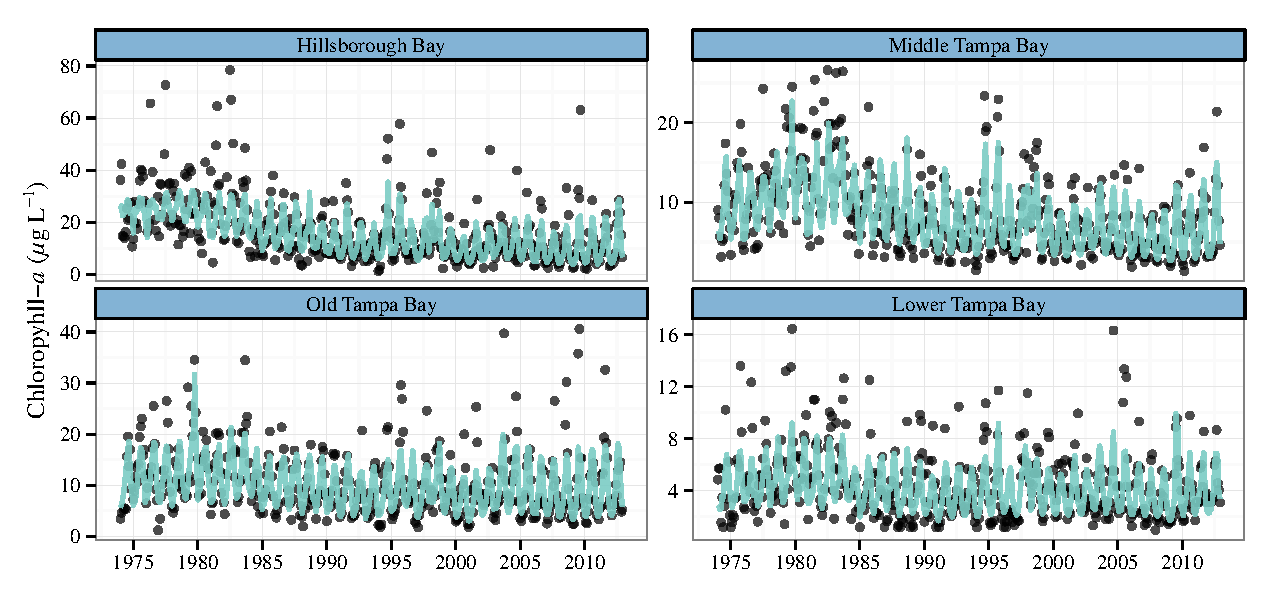
\includegraphics[width=\linewidth]{fig/predvals-1} 

}

\caption[Predicted and observed monthly chlorophyll by segment]{Predicted and observed monthly chlorophyll by segment.}\label{fig:predvals}
\end{figure}


\end{frame}

%%%%%%
\begin{frame}{\textbf{Case 2: Florida estuaries}}{\textbf{Evaluating long-term chlorophyll datasets}}
Because the model is dynamic, we have parameters describing the relationship of chlorophyll with other factors specific to different time periods \\~\\
\begin{columns}[T]
\begin{column}{0.45\textwidth}


{\centering 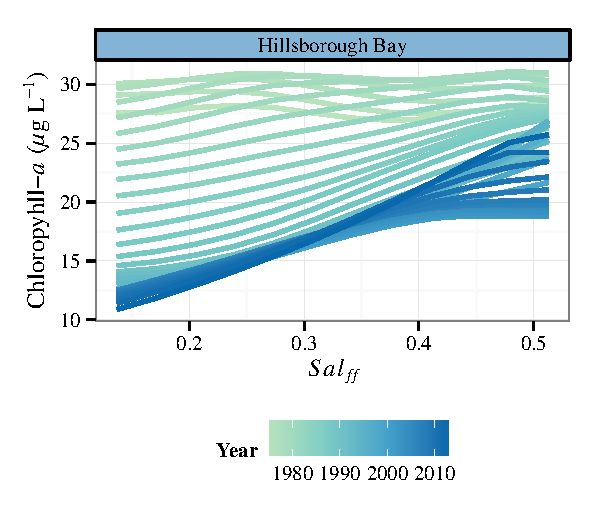
\includegraphics[width=\maxwidth]{fig/hill-1} 

}



\end{column}
\begin{column}{0.45\textwidth}
\begin{itemize}
\item Early period (light blue) - point-sources
\item Late period (dark blue) - non-point sources
\item Chlorophyll shows increasing response to freshwater input in recent years
\end{itemize}
\end{column}
\end{columns}
\end{frame}

%%%%%%
\begin{frame}{\textbf{Case 2: Florida estuaries}}{\textbf{Evaluating long-term chlorophyll datasets}}
\onslide<+->
What does this mean for Tampa Bay and elsewhere?\\~\\
\begin{itemize}
\item Predictions followed observed chlorophyll -- but increased clarity in the description
\item More detailed evaluation of trends allows greater insight into drivers of change\\~\\
\end{itemize}
\onslide<+->
The model parameters show us a picture...
\centerline{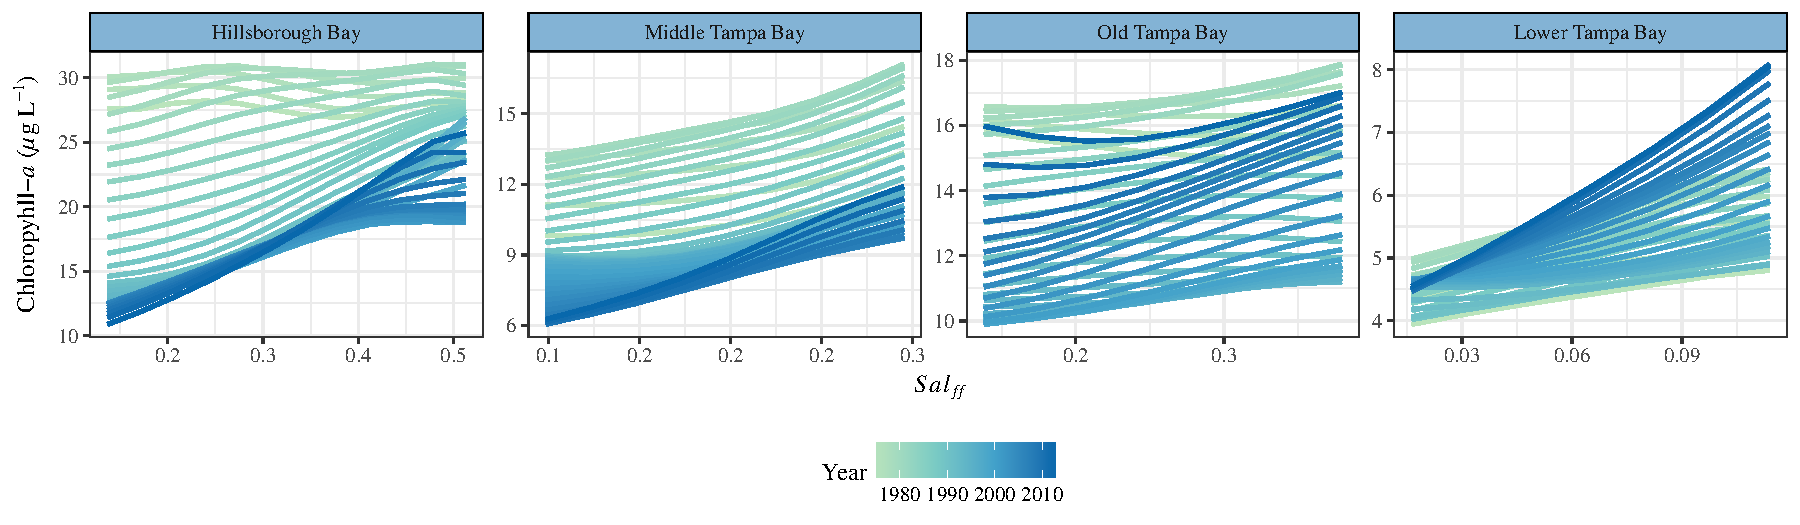
\includegraphics[width = \textwidth]{fig/title_plo.pdf}}
\end{frame}

\section{Case 3: Open-source tools}
%%%%%%
\begin{frame}{\textbf{Case 3: Open-source science}}{\textbf{Analysis tools for water quality data}}
\onslide<+->
Progress in science is incremental and builds on past work\\~\\
This requires accurate reproduction of methods\\~\\
The ability to reproduce methods will always be a challenge...\\~\\
\onslide<+->
...digital tools have proliferated to \emtxt{facilitate sharing}\\~\\
\begin{columns}
\begin{column}{0.25\textwidth}
\centerline{
\includegraphics[width = \textwidth]{fig/Rlogo.png}}
\end{column}
\begin{column}{0.25\textwidth}
\centerline{
\includegraphics[width = \textwidth]{fig/RStudio.png}}
\end{column}
\begin{column}{0.25\textwidth}
\centerline{
\includegraphics[width = \textwidth]{fig/knit-logo.png}}
\end{column}
\begin{column}{0.25\textwidth}
\centerline{
\includegraphics[width = \textwidth]{fig/octocat.png}}
\end{column}
\end{columns}
\end{frame}

%%%%%%
\begin{frame}{\textbf{Case 3: Open-source science}}{\textbf{Analysis tools for water quality data}}
The NERRS System-Wide Monitoring Program...\\~\\
\centerline{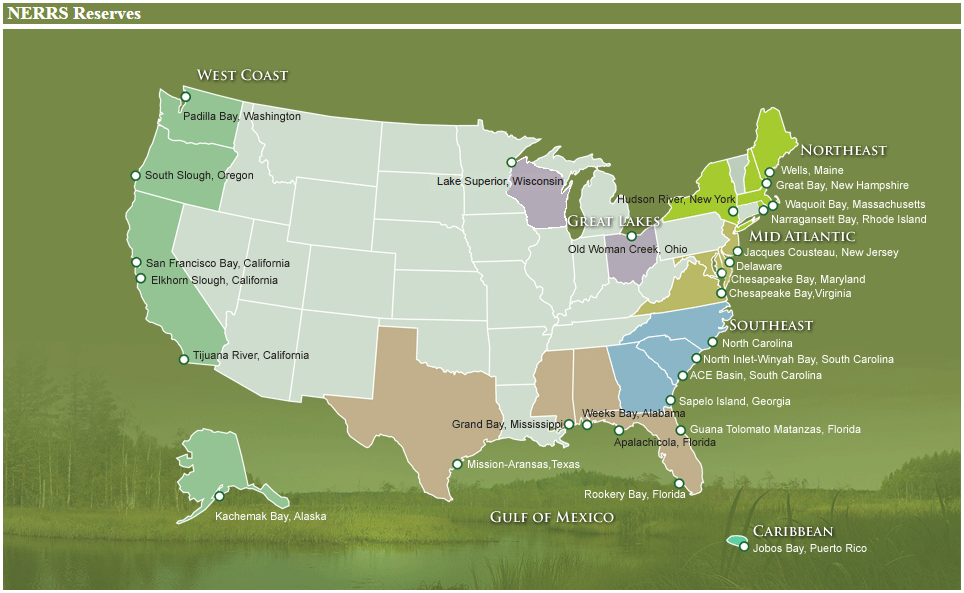
\includegraphics[width = 0.8\textwidth]{fig/NERRS_locations.png}}
\end{frame}

%%%%%%
\begin{frame}{\textbf{Case 3: Open-source science}}{\textbf{Analysis tools for water quality data}}
\onslide<+->
The SWMP database and others like it represent incredible opportunities to further our knowledge of natural systems...\\~\\
...including the effects of eutrophication \\~\\
\onslide<+->
\emtxt{Problem:} These data are numerous and not easily compared\\~\\
\emtxt{Solution:} Develop open-source tools that address the challenges of large-scale comparative analyses with continuous monitoring data\\~\\
\onslide<+->
The benefits include:
\begin{itemize}
\item Free for use by anyone
\item Free to collaborate
\item Facilitation of analysis with `under-the-hood' functionality
\end{itemize}
\end{frame}

%%%%%%
\begin{frame}[t]{\textbf{Case 3: Open-source science}}{\textbf{Analysis tools for water quality data}}
Each reserve has fixed, continuous monitoring stations for \emtxt{water quality} (15 min), \emtxt{meteorology} (15 min), and \emtxt{nutrients} (monthly)\\~\\
As of this month, $>$ 60 million records available online\\~\\
Raw data look like this:\\~\\
\centerline{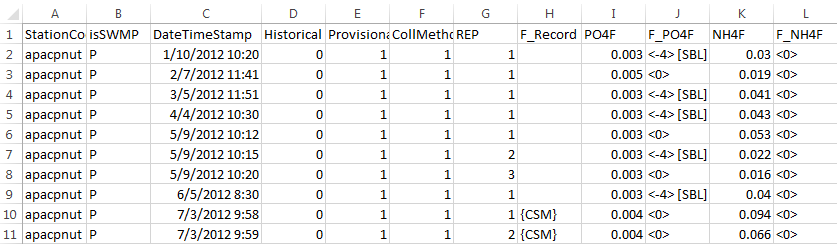
\includegraphics[width = 0.9\textwidth]{fig/qaqc_ex.png}}
\end{frame}

%%%%%%
\begin{frame}{\textbf{Case 3: Open-source science}}{\textbf{Analysis tools for water quality data}}
\centerline{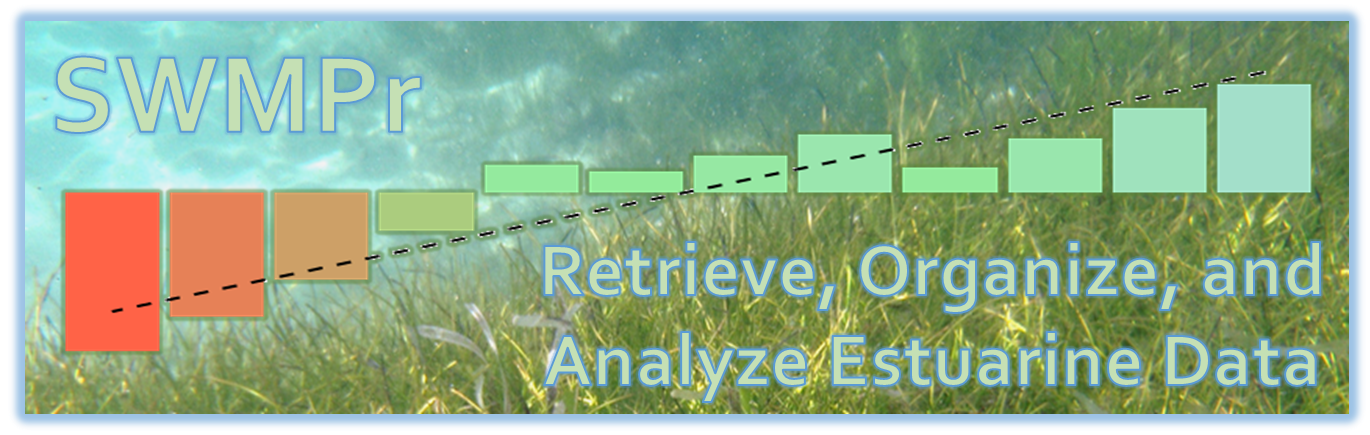
\includegraphics[width = 0.8\textwidth]{fig/swmpr_logo.png}}
\vspace{0.15in}
\emtxt{SWMPr} is a freely available package for use with R \\~\\
\begin{itemize}
\item \emtxt{Retrieve} SWMP data for any site and date combination
\item \emtxt{Organize} the data using standard pre-processing techniques
\item \emtxt{Analyze} the data using a suite of exploratory and graphical analysis tools
\end{itemize}
\end{frame}

%%%%%%
\begin{frame}{\textbf{Case 3: Open-source science}}{\textbf{Analysis tools for water quality data}}
\href{https://swmprats.net}{SWMPrats.net}: \emtxt{S}ystem-\emtxt{W}ide \emtxt{M}onitoring \emtxt{P}rogram \emtxt{R}esources for the \emtxt{A}nalysis of \emtxt{T}ime \emtxt{S}eries \\~\\
\centerline{\fbox{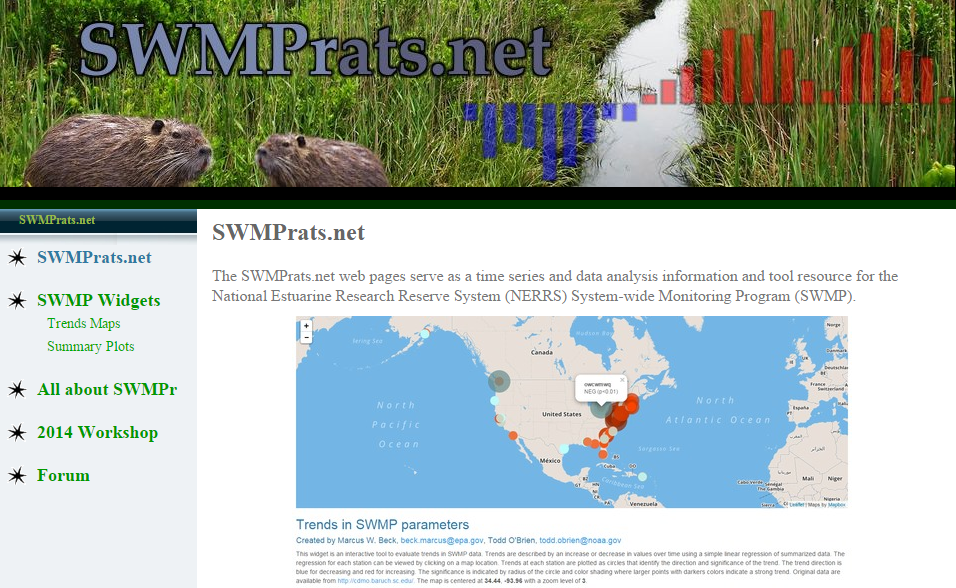
\includegraphics[width = 0.75\textwidth]{fig/swmprats_home.png}}}
\end{frame}

%%%%%%
\begin{frame}{\textbf{Case 3: Open-source science}}{\textbf{Analysis tools for water quality data}}
Two online applications can help visualize trends \\~\\
\begin{columns}[t]
\begin{column}{0.45\textwidth}
\centerline{\emtxt{\href{https://beckmw.shinyapps.io/swmp_summary}{Summary plots}}}
\centerline{\fbox{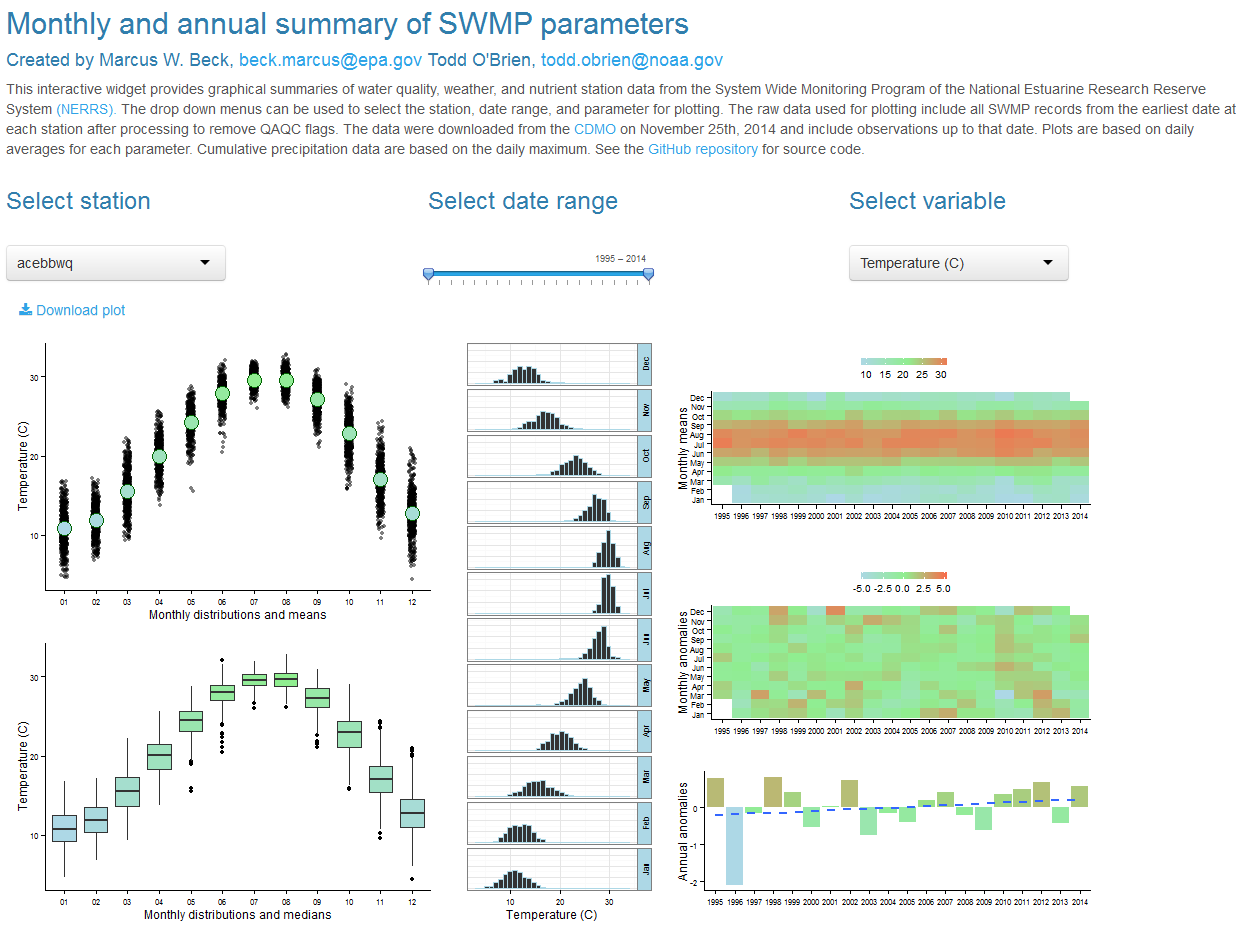
\includegraphics[width = 0.9\textwidth]{fig/swmp_summary.png}}}
\end{column}
\begin{column}{0.45\textwidth}
\centerline{\emtxt{\href{https://beckmw.shinyapps.io/swmp_comp}{Trends map}}}
\centerline{\fbox{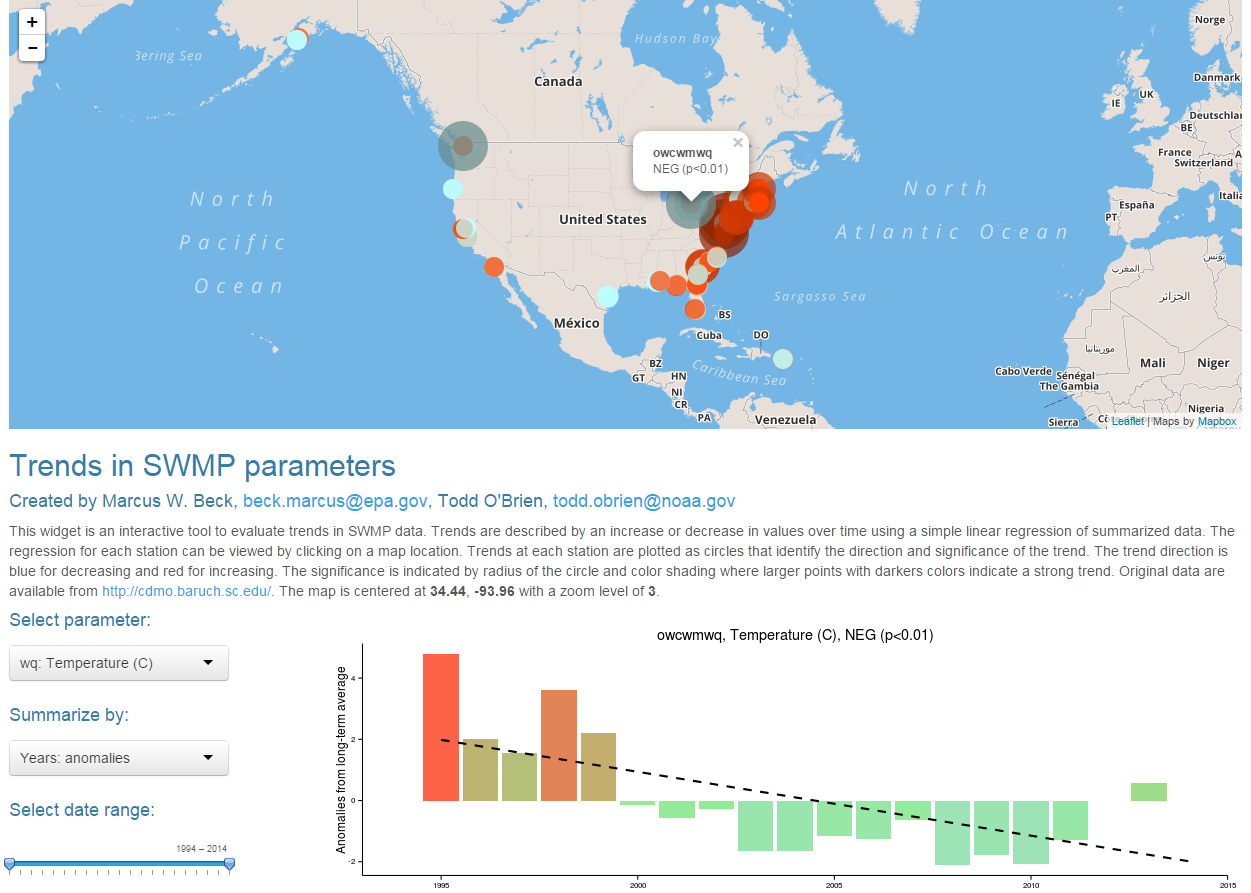
\includegraphics[width = 0.935\textwidth]{fig/swmp_comp.png}}}
\end{column}
\end{columns}
\end{frame}

%%%%%%
\begin{frame}{\textbf{Case 3: Open-source science}}{\textbf{Analysis tools for water quality data}}
\onslide<+->
Tools in the SWMPr package have facilitated comparative analyses of millions of water quality records from NERRS \\~\\
These tools can help improve our understanding of nutrient pollution and eutrophication \\~\\
\onslide<+->
Potential for many other applications... actively being developed \\~\\
\begin{columns}
\begin{column}{0.25\textwidth}
\centerline{
\includegraphics[width = \textwidth]{fig/Rlogo.png}}
\end{column}
\begin{column}{0.25\textwidth}
\centerline{
\includegraphics[width = \textwidth]{fig/RStudio.png}}
\end{column}
\begin{column}{0.25\textwidth}
\centerline{
\includegraphics[width = \textwidth]{fig/knit-logo.png}}
\end{column}
\begin{column}{0.25\textwidth}
\centerline{
\includegraphics[width = \textwidth]{fig/octocat.png}}
\end{column}
\end{columns}
\end{frame}

%%%%%%
\begin{frame}{\textbf{Conclusions}}
Our ability to \emtxt{share}, \emtxt{reproduce}, and \emtxt{collaborate} is essential \\~\\
\emtxt{SWMPr package:} \href{https://github.com/fawda123/SWMPr}{https://github.com/fawda123/SWMPr} \\~\\
\emtxt{Summaries of SWMP parameters:} \href{https://beckmw.shinyapps.io/swmp_summary}{https://beckmw.shinyapps.io/swmp\_summary} \\~\\
\emtxt{Trends in SWMP parameters:} \href{https://beckmw.shinyapps.io/swmp_comp}{https://beckmw.shinyapps.io/swmp\_comp} \\~\\
\emtxt{This presentation:} \href{https://github.com/fawda123/ncea_pres}{https://github.com/fawda123/ncea\_pres} \\~\\
\emtxt{Github}: \href{https://github.com/fawda123/}{github.com/fawda123/} \\~\\
\emtxt{Blog}: \href{http://beckmw.wordpress.com/}{beckmw.wordpress.com/}
\end{frame}

%%%%%%
\begin{frame}
Acknowledgments:\\~\\
\begin{columns}
\begin{column}{0.8\textwidth}
{\footnotesize
Research staff and employees at USEPA Gulf Ecology Division - especially J. Hagy, M. Murrell\\~\\
Field staff and data managers at Hillsborough County Environmental Protection Commission\\~\\
Research coordinators, technicians, and field staff of the National Estuarine Research Reserve System}\\~\\
\end{column}
\begin{column}{0.2\textwidth}
\end{column}
\end{columns}
\vfill
Funding sources and contact:\\~\\
\begin{columns}
\begin{column}{0.5\textwidth}
\centerline{
\includegraphics[width=0.4\linewidth]{fig/epa_logo.png}}
\end{column}
\begin{column}{0.5\textwidth}
\scriptsize
\href{mailto:beck.marcus@epa.gov}{beck.marcus@epa.gov} \\~\\
Phone: 8509342480
\end{column}
\end{columns}
\vspace{0.2in}
\end{frame}

%%%%%%
\section{References}
\begin{frame}[allowframebreaks,t]{\textbf{References}}
\tiny
\setbeamertemplate{bibliography item}{}
\bibliographystyle{apalike_mine}
\bibliography{refs}
\end{frame}

\end{document}
